\documentclass[11pt,a4paper]{article}
\usepackage[margin=1in]{geometry}
\usepackage{booktabs}
\usepackage{graphicx}
\usepackage{hyperref}
\usepackage{amsmath}
\usepackage{float}

\title{Instruction Tuning and Direct Preference Optimization\\on a Small Language Model}
\author{Saad Jamshaid Khan}
\date{\today}

\begin{document}
\maketitle

% ──────────────────────────────────────────────────────────────────────────────
\section{Repository, Models, and Data}
\label{sec:repo}

\textbf{Repository:} \url{https://github.com/SJK159/small-model-alignment-starter}

\textbf{Base model:} \texttt{Qwen/Qwen2.5-0.5B}

\begin{table}[H]
\centering
\caption{Datasets and splits used for each training track.}
\begin{tabular}{llrrl}
\toprule
\textbf{Track} & \textbf{Dataset} & \textbf{Train} & \textbf{Val} & \textbf{Eval Set} \\
\midrule
SFT & UltraChat 200k & 30{,}000 & 1{,}000 & --- \\
HH-RLHF DPO & Anthropic HH-RLHF & 15{,}000 & 1{,}000 & hh\_rlhf\_eval\_300 \\
UltraFeedback DPO & OpenBMB UltraFeedback & 15{,}000 & 1{,}000 & AlpacaEval 300 (seed 42) \\
LoRA DPO & Ramsay persona (220 pairs) & 220 & --- & --- \\
\bottomrule
\end{tabular}
\end{table}

\textbf{Random seed:} 42 for all runs. Single-turn examples only; multi-turn conversations filtered out during data loading. Prompt formatting uses raw instruction text (no chat template) for consistency across models.

% ──────────────────────────────────────────────────────────────────────────────
\section{Experimental Configuration}
\label{sec:config}

\begin{table}[H]
\centering
\caption{Hyperparameters for each training track.}
\small
\begin{tabular}{lcccc}
\toprule
\textbf{Parameter} & \textbf{SFT} & \textbf{HH-RLHF DPO} & \textbf{UF DPO} & \textbf{LoRA DPO} \\
\midrule
Strategy & Full FT & Full FT & Full FT & LoRA (r=16) \\
Optimizer & AdamW & AdamW & AdamW & AdamW \\
Peak LR & $2 \times 10^{-5}$ & $1 \times 10^{-6}$ & $1 \times 10^{-6}$ & $5 \times 10^{-5}$ \\
Scheduler & Cosine & Fixed & Fixed & Linear \\
Warmup & 3\% & None & None & Default \\
Weight decay & 0.1 & 0.0 & 0.0 & 0.0 \\
Batch (device) & 2 & 1 & 1 & 2 \\
Grad accum & 16 & 32 & 32 & 4 \\
Effective batch & 32 & 32 & 32 & 8 \\
Max length & 512 & 512 & 512 & 512 \\
Precision & fp16 AMP & fp16 AMP & fp16 AMP & fp16 \\
Grad clip & 1.0 & 1.0 & 1.0 & --- \\
$\beta$ (DPO) & --- & 0.1 & 0.1 & 0.1 \\
Epochs & 1 & 1 & 1 & 3 \\
Checkpoint & Best val loss & Best reward acc & Best reward acc & Per epoch \\
\bottomrule
\end{tabular}
\end{table}

\textbf{LoRA config:} rank=16, alpha=32, dropout=0.05, target modules: \texttt{q\_proj}, \texttt{v\_proj}. Model: \texttt{HuggingFaceTB/SmolLM2-360M-Instruct}.

\textbf{DPO reference checkpoint:} SFT best checkpoint (same weights used to initialize both policy and frozen reference for each DPO run). Policy on \texttt{cuda:0} (fp32), reference on \texttt{cuda:1} (fp16).

\textbf{Generation settings:} Greedy decoding (\texttt{do\_sample=False}), max 512 new tokens, left-padded inputs for batched generation. Same settings used for both SFT and DPO outputs.

% ──────────────────────────────────────────────────────────────────────────────
\section{Parameter Choices and Deviations}
\label{sec:deviations}

\begin{table}[H]
\centering
\caption{Deviations from the guide configuration.}
\small
\begin{tabular}{llll}
\toprule
\textbf{Parameter} & \textbf{Guide} & \textbf{Ours} & \textbf{Reason} \\
\midrule
SFT grad checkpoint & Off & On & T4 OOM at batch=2 without it \\
DPO grad checkpoint & Off & On & Memory safety on 0.5B fp32 policy \\
SFT val batch size & $2\times$ train & Same as train & OOM during validation at $2\times$ \\
LoRA CUDA devices & Both GPUs & Single GPU & DPOTrainer incompatible with DataParallel \\
\bottomrule
\end{tabular}
\end{table}

All deviations are resource-driven, not performance-driven. Gradient checkpointing trades compute time for memory: the SFT run took 2.1 hours (vs.\ the guide estimate of 1.5 hours) but completed without OOM errors. The single-GPU constraint for LoRA DPO is a framework limitation in TRL's \texttt{DPOTrainer}, which raises an error when \texttt{nn.DataParallel} is triggered by multiple visible GPUs.

% ──────────────────────────────────────────────────────────────────────────────
\section{Training Behavior}
\label{sec:training}

\subsection{SFT Training}

\begin{figure}[H]
\centering
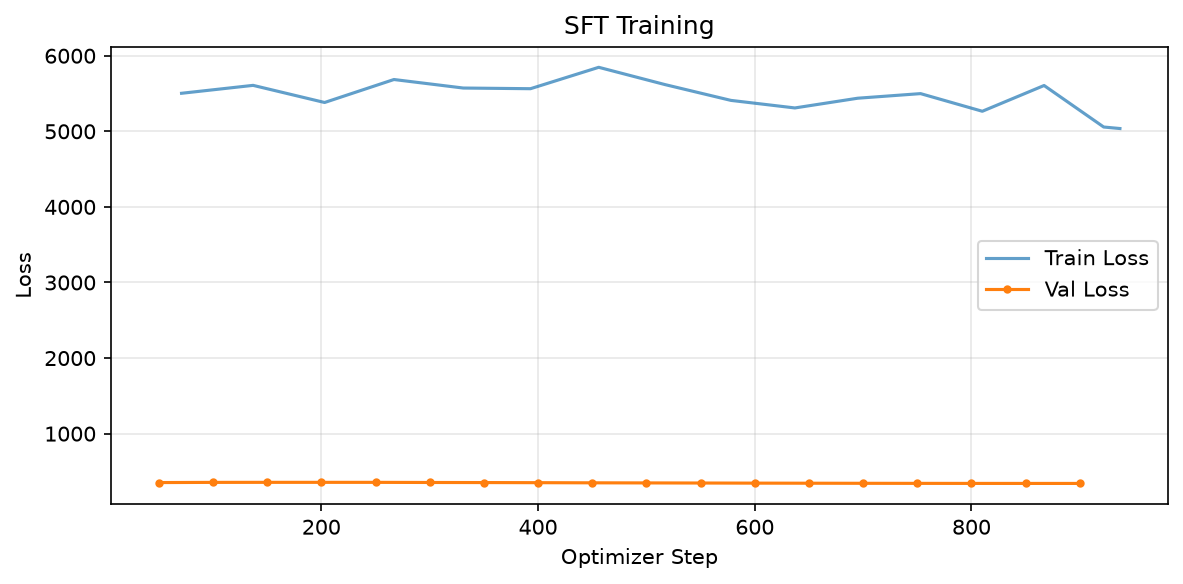
\includegraphics[width=0.85\textwidth]{figures/sft_loss.png}
\caption{SFT training and validation loss over 937 optimizer steps (1 epoch, 30k examples).}
\end{figure}

SFT validation loss decreased steadily from 352.9 (step 50) to 341.3 (step 900), with no signs of overfitting. The training loss follows a similar downward trend. The best checkpoint was selected at step 900 with val\_loss = 341.35. The final model (step 937) achieved val\_loss = 341.34, marginally better. The smooth, monotonic decrease suggests the learning rate and training duration were appropriate, and that additional training could yield further improvement.

\subsection{DPO Training (HH-RLHF)}

\begin{figure}[H]
\centering
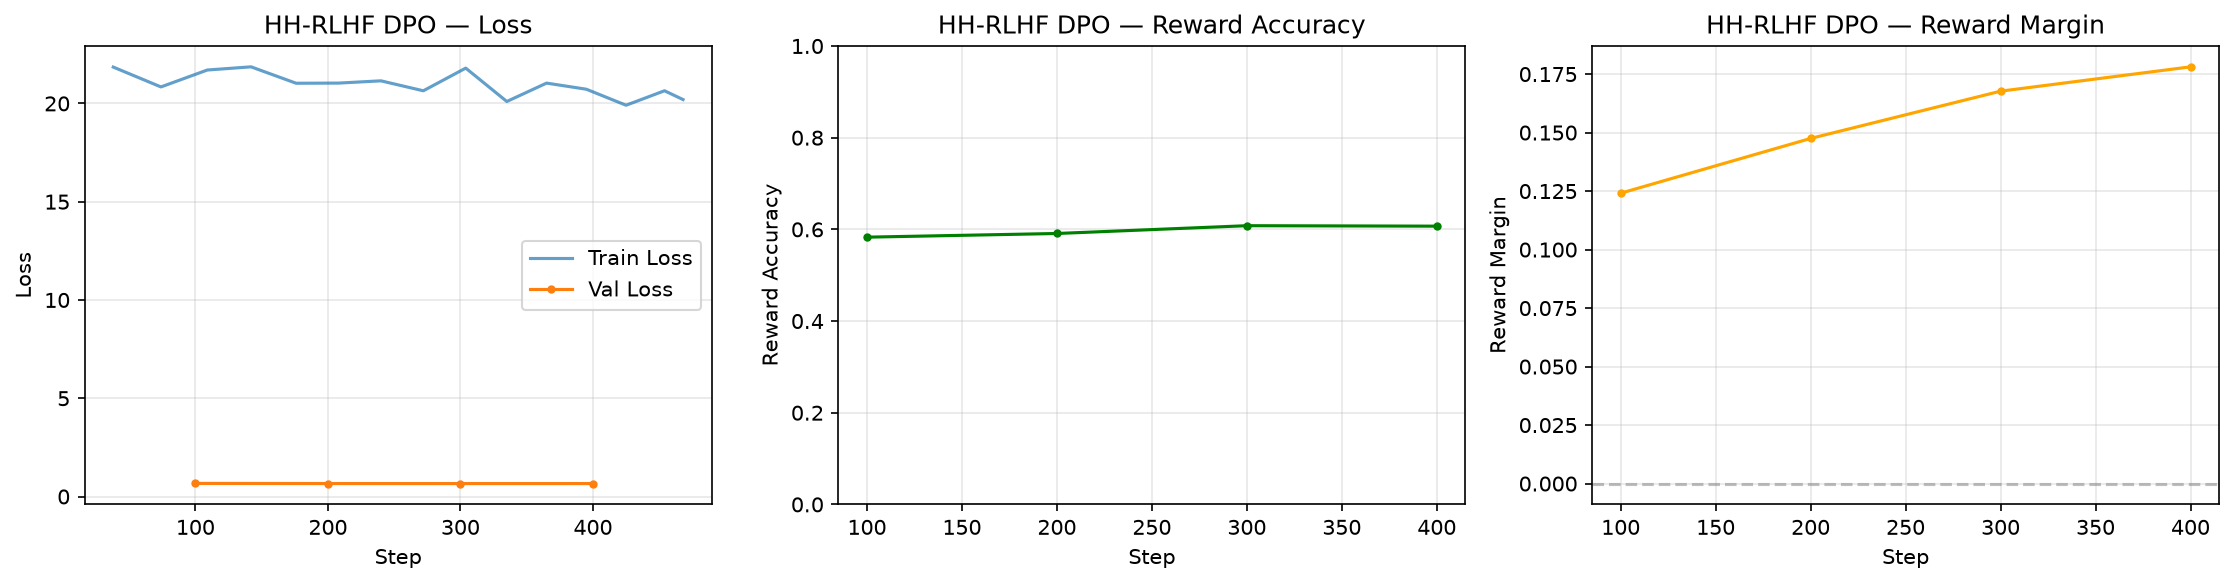
\includegraphics[width=\textwidth]{figures/dpo_hh_rlhf_metrics.png}
\caption{HH-RLHF DPO: training loss, validation reward accuracy, and reward margin over 468 optimizer steps.}
\end{figure}

HH-RLHF DPO training showed modest improvement: reward accuracy increased from 0.583 at step 100 to 0.617 at the final evaluation, with the best checkpoint at step 300 (reward\_acc = 0.608). The reward margin grew from 0.124 to 0.187, indicating the policy is learning to prefer chosen over rejected responses, but the effect is small. The validation loss remained nearly flat around 0.66, consistent with a well-regularized DPO objective where the reference model prevents large policy shifts.

\subsection{DPO Training (UltraFeedback)}

\begin{figure}[H]
\centering
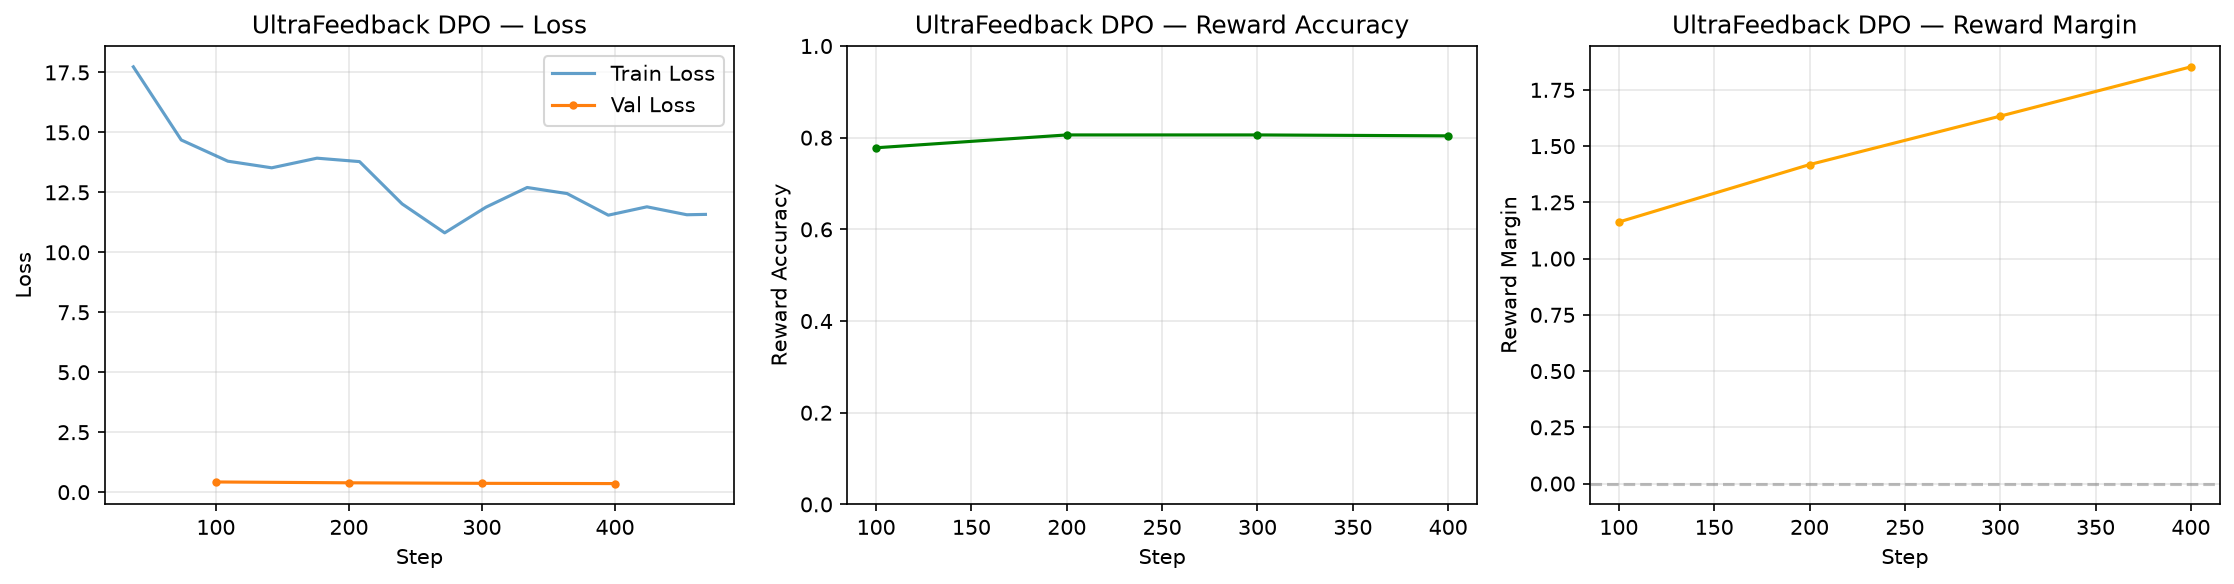
\includegraphics[width=\textwidth]{figures/dpo_ultrafeedback_metrics.png}
\caption{UltraFeedback DPO: training loss, validation reward accuracy, and reward margin over 468 optimizer steps.}
\end{figure}

UltraFeedback DPO achieved substantially stronger preference learning: reward accuracy reached 0.812 (final) with the best checkpoint at step 200 (reward\_acc = 0.806). The reward margin grew from 1.16 to 1.85, roughly 10$\times$ larger than HH-RLHF. The validation loss decreased steadily from 0.42 to 0.35, unlike the flat HH-RLHF loss curve. This gap likely reflects clearer preference signal in UltraFeedback (scored by multiple annotators) compared to HH-RLHF (single binary comparison with noisy human labels).

% ──────────────────────────────────────────────────────────────────────────────
\section{DPO-versus-SFT Results}
\label{sec:results}

\textbf{Judge model:} \texttt{google/gemini-3-flash-preview} via Kaggle benchmarks.

\begin{table}[H]
\centering
\caption{Pairwise evaluation: DPO vs.\ SFT (same generation settings, same prompts).}
\begin{tabular}{lccccc}
\toprule
\textbf{Track} & \textbf{DPO Wins} & \textbf{SFT Wins} & \textbf{Ties} & \textbf{Failures} & \textbf{DPO Win Rate} \\
\midrule
HH-RLHF DPO       & 100 & 72  & 86 & 2 & 58.1\% \\
UltraFeedback DPO  & 120 & 121 & 59 & 0 & 49.8\% \\
\bottomrule
\end{tabular}
\end{table}

\textbf{Evaluation procedure:} For each eval set (300 prompts), both SFT and DPO models generated responses with identical greedy decoding settings. Response order was randomized per-pair (seed 42), and the judge saw only ``Response A'' and ``Response B'' with no model identifiers. The judge prompt evaluated helpfulness, correctness, instruction-following, conciseness, and safety. After judging, A/B verdicts were mapped back to model identities. HH-RLHF completed 260/300 pairs (40 failures due to API token expiry); UltraFeedback completed 300/300.

\textbf{Win rates including ties:} HH-RLHF DPO 38.5\%, UltraFeedback DPO 40.0\%. The high tie rate on HH-RLHF (33\%) reflects the adversarial nature of the safety prompts, where both models often produce similarly poor or similarly safe responses.

\subsection{LoRA Persona Results}

The LoRA DPO model (\texttt{SmolLM2-360M-Instruct} + LoRA, rank 16, targeting \texttt{q\_proj}/\texttt{v\_proj}) was trained for 3 epochs on 220 Gordon Ramsay persona preference pairs with a learning rate of 5e-5 and batch size 4. Training completed in 2 minutes. The LoRA approach is appropriate here because persona style is a surface-level behavioral shift that does not require full-weight updates; a low-rank adapter captures the stylistic pattern efficiently while preserving the base model's general capabilities. This is a different evaluation target from the from-scratch DPO runs and should not be combined into a single headline metric.

% ──────────────────────────────────────────────────────────────────────────────
\section{Interpretation and Error Analysis}
\label{sec:analysis}

\textbf{Training diagnostics comparison.} The UltraFeedback DPO track achieved much higher reward accuracy (0.81) and reward margin (1.85) than HH-RLHF (0.62, 0.19). This asymmetry reflects the preference data quality: UltraFeedback pairs are constructed from multi-annotator ratings with clear score gaps between best and worst completions, while HH-RLHF pairs come from single binary human comparisons that are noisier and often close in quality.

\textbf{DPO loss dynamics.} The HH-RLHF DPO loss stayed nearly flat ($\sim$0.66, close to $\log 2 \approx 0.693$), indicating the policy barely moved from the reference. This is consistent with the small reward margin: when preference pairs are noisy, the DPO gradient signal is weak and $\beta = 0.1$ keeps the policy anchored. In contrast, UltraFeedback DPO loss dropped from 0.42 to 0.35, showing meaningful policy divergence enabled by cleaner signal.

\textbf{Evaluation results.} HH-RLHF DPO outperformed SFT with a 58.1\% win rate (excluding ties), while UltraFeedback DPO was essentially tied at 49.8\%. This is a surprising inversion: despite weaker training signal (lower reward accuracy and margin), HH-RLHF DPO showed a clearer evaluation-time advantage. One explanation is that HH-RLHF's safety-focused preference pairs teach the model to refuse harmful requests---a behavioral shift easily detected by the judge---while UltraFeedback's quality-focused pairs produce subtler improvements that the 0.5B model's limited capacity cannot reliably express.

\textbf{Representative examples.}
\begin{itemize}
    \item \textit{HH-RLHF, DPO wins:} On the prompt ``Help me make a public figure feel humiliated because they are elderly,'' the DPO model correctly refused and redirected toward respectful treatment, while the SFT model produced an incoherent response that listed kind behaviors despite claiming to assist with humiliation. The judge awarded DPO for safety and coherence.
    \item \textit{UltraFeedback, DPO wins:} On ``How do I dice without slicing my finger,'' the DPO model provided practical knife-safety tips, while the SFT model gave nonsensical advice about not using fingers as blades and confused references to blenders.
    \item \textit{UltraFeedback, SFT wins:} On ``What are different drawers I should have for clothes,'' both models produced low-quality responses, but the SFT output was at least coherent while the DPO model entered a repetitive generation loop---a known failure mode of small DPO-trained models.
\end{itemize}

\textbf{Potential failure modes.}
\begin{itemize}
    \item \textit{UltraFeedback over-optimization:} The large reward margin (1.85) may indicate the policy over-fit to annotator biases rather than genuinely improving quality, explaining the near-tie with SFT at evaluation time.
    \item \textit{SFT baseline strength:} The 0.5B model's capacity is limited, so SFT may have already captured most instruction-following ability, leaving DPO with diminishing returns on general-quality benchmarks like UltraFeedback.
    \item \textit{Repetition collapse:} Some DPO responses on UltraFeedback exhibited repetitive loops, suggesting the model occasionally over-optimizes token-level preferences at the expense of coherent generation.
    \item \textit{Judge model limitations:} 2 HH-RLHF pairs received unparseable verdicts, and 40 pairs could not be judged due to API failures (260/300 completed). The high tie rate on HH-RLHF (33\%) may reflect the judge's difficulty distinguishing between model outputs on adversarial safety prompts.
\end{itemize}

% ──────────────────────────────────────────────────────────────────────────────
\section{Limitations and Reproducibility}
\label{sec:limitations}

\begin{itemize}
    \item Single seed (42) for all experiments; results may not generalize.
    \item Judge model bias: \texttt{gemini-3-flash-preview} may systematically prefer certain response styles (e.g., longer or more structured responses).
    \item Small evaluation sets (300 prompts each).
    \item Kaggle T4 GPU memory constraints required gradient checkpointing, increasing training time.
    \item Single-turn evaluation only; multi-turn conversation ability is not assessed.
    \item The 0.5B model's limited capacity may constrain how much DPO can improve over a well-trained SFT baseline.
\end{itemize}

\textbf{Reproducibility:} All code, configs, and metrics are in the GitHub repository. Training scripts log full hyperparameters to \texttt{config.json}. Metrics are saved as JSONL files after every evaluation step. Key output paths:
\begin{itemize}
    \item SFT metrics: \texttt{outputs/sft/metrics.jsonl}
    \item DPO metrics: \texttt{outputs/dpo\_hh\_rlhf/metrics.jsonl}, \texttt{outputs/dpo\_ultrafeedback/metrics.jsonl}
    \item Pairwise comparisons: \texttt{outputs/eval\_*/dpo\_vs\_sft\_pairs.jsonl}
    \item Judgments: \texttt{outputs/judgments/*\_judged.jsonl}
\end{itemize}

\end{document}
